%!TEX TS-program = xelatex
%!TEX root = ../../maxwell2018thesis.tex

\chapter[The Complex Searcher Model and Stopping Strategies]{The Complex Searcher Model\\and Stopping Strategies}\label{chap:csm}
In Part~\ref{part:intro}, we provided a comprehensive overview of the current state-of-the-art of user modelling within the field of~\gls{acr:iir} -- and stopping within search. In this chapter, we present an improvement on the current state-of-the-art, providing an outline of the main conceptual and theoretical contributions of this thesis, which include proposals of:

\vspace*{-2mm}
\begin{itemize}
    \item[\blueboxbold{(i)}]{a more complex and realistic user model -- the~\glsfirst{acr:csm} -- that captures the key interactions that take place during an~\gls{acr:iir} session (Section~\ref{sec:csm:csm}); and}
    \item[\blueboxbold{(ii)}]{an enumeration of a number of \emph{stopping strategies} that we will be evaluating (Section~\ref{sec:csm:stopping}).}
\end{itemize}
\vspace*{-2mm}

These outlines provide the foundations for the subsequent contributory chapters of this thesis that aim to both evaluate the quality of the proposed~\gls{acr:csm}, and the effectiveness of the proposed stopping strategies. Each of the stopping strategies that are proposed in this chapter are operationalised from a number of stopping heuristics defined in the literature, reviewed previously in Chapter~\ref{chap:stopping_background}. To complement the above, we also provide in this chapter \blueboxbold{(iii)} a high level description of the basic methodology we employ in subsequent chapters of this thesis (Section~\ref{sec:csm:methodology}).

\section{The Complex Searcher Model}\label{sec:csm:csm}
The~\glsfirst{acr:csm} is a high level, conceptual model of the search process that captures the key processes and decisions that are taken by a searcher during the information seeking process. Illustrated in Figure~\ref{fig:csm}, the~\gls{acr:csm} is an amalgamation and further development of prior, established models that capture the information seeking process. Discussed previously in Section~\ref{sec:stopping_background:models:conceptual}, prime examples of prior models include the Markov-based approach by~\cite{baskaya2013behavioural_factors}, and the searcher model proposed by~\cite{thomas2014modelling_behaviour}. These models (along with others) are in broad agreement with the general sequence of events that searchers undertake -- from issuing a query to examining documents for relevance. Refer to Figures~\ref{fig:baskaya_model_flow} and~\ref{fig:thomas_model} on pages~\pageref{fig:baskaya_model_flow} and~\pageref{fig:thomas_model} respectively for illustrations of the two aforementioned models.

Given the \emph{baseline models} outlined above and in Section~\ref{sec:stopping_background:models:conceptual}, the~\gls{acr:csm} offers a number of advancements in modelling the information seeking process. In this section, we outline:

\begin{itemize}
    \item{the \emph{flow} of the model, explaining the different steps and decisions that a searcher undertakes (Section~\ref{sec:csm:csm:flow});}
    \item{the different \emph{stopping decision points} of the model (Section~\ref{sec:csm:csm:stopping}); and}
    \item{the \emph{assumptions} that are made as part of the~\gls{acr:csm} (Section~\ref{sec:csm:csm:assumptions}).}
\end{itemize}

We begin however with an overview of the key advancements that the~\gls{acr:csm} provides over existing models of the information seeking process.

\begin{figure}[t!]
    \centering
    \resizebox{1\hsize}{!}{
    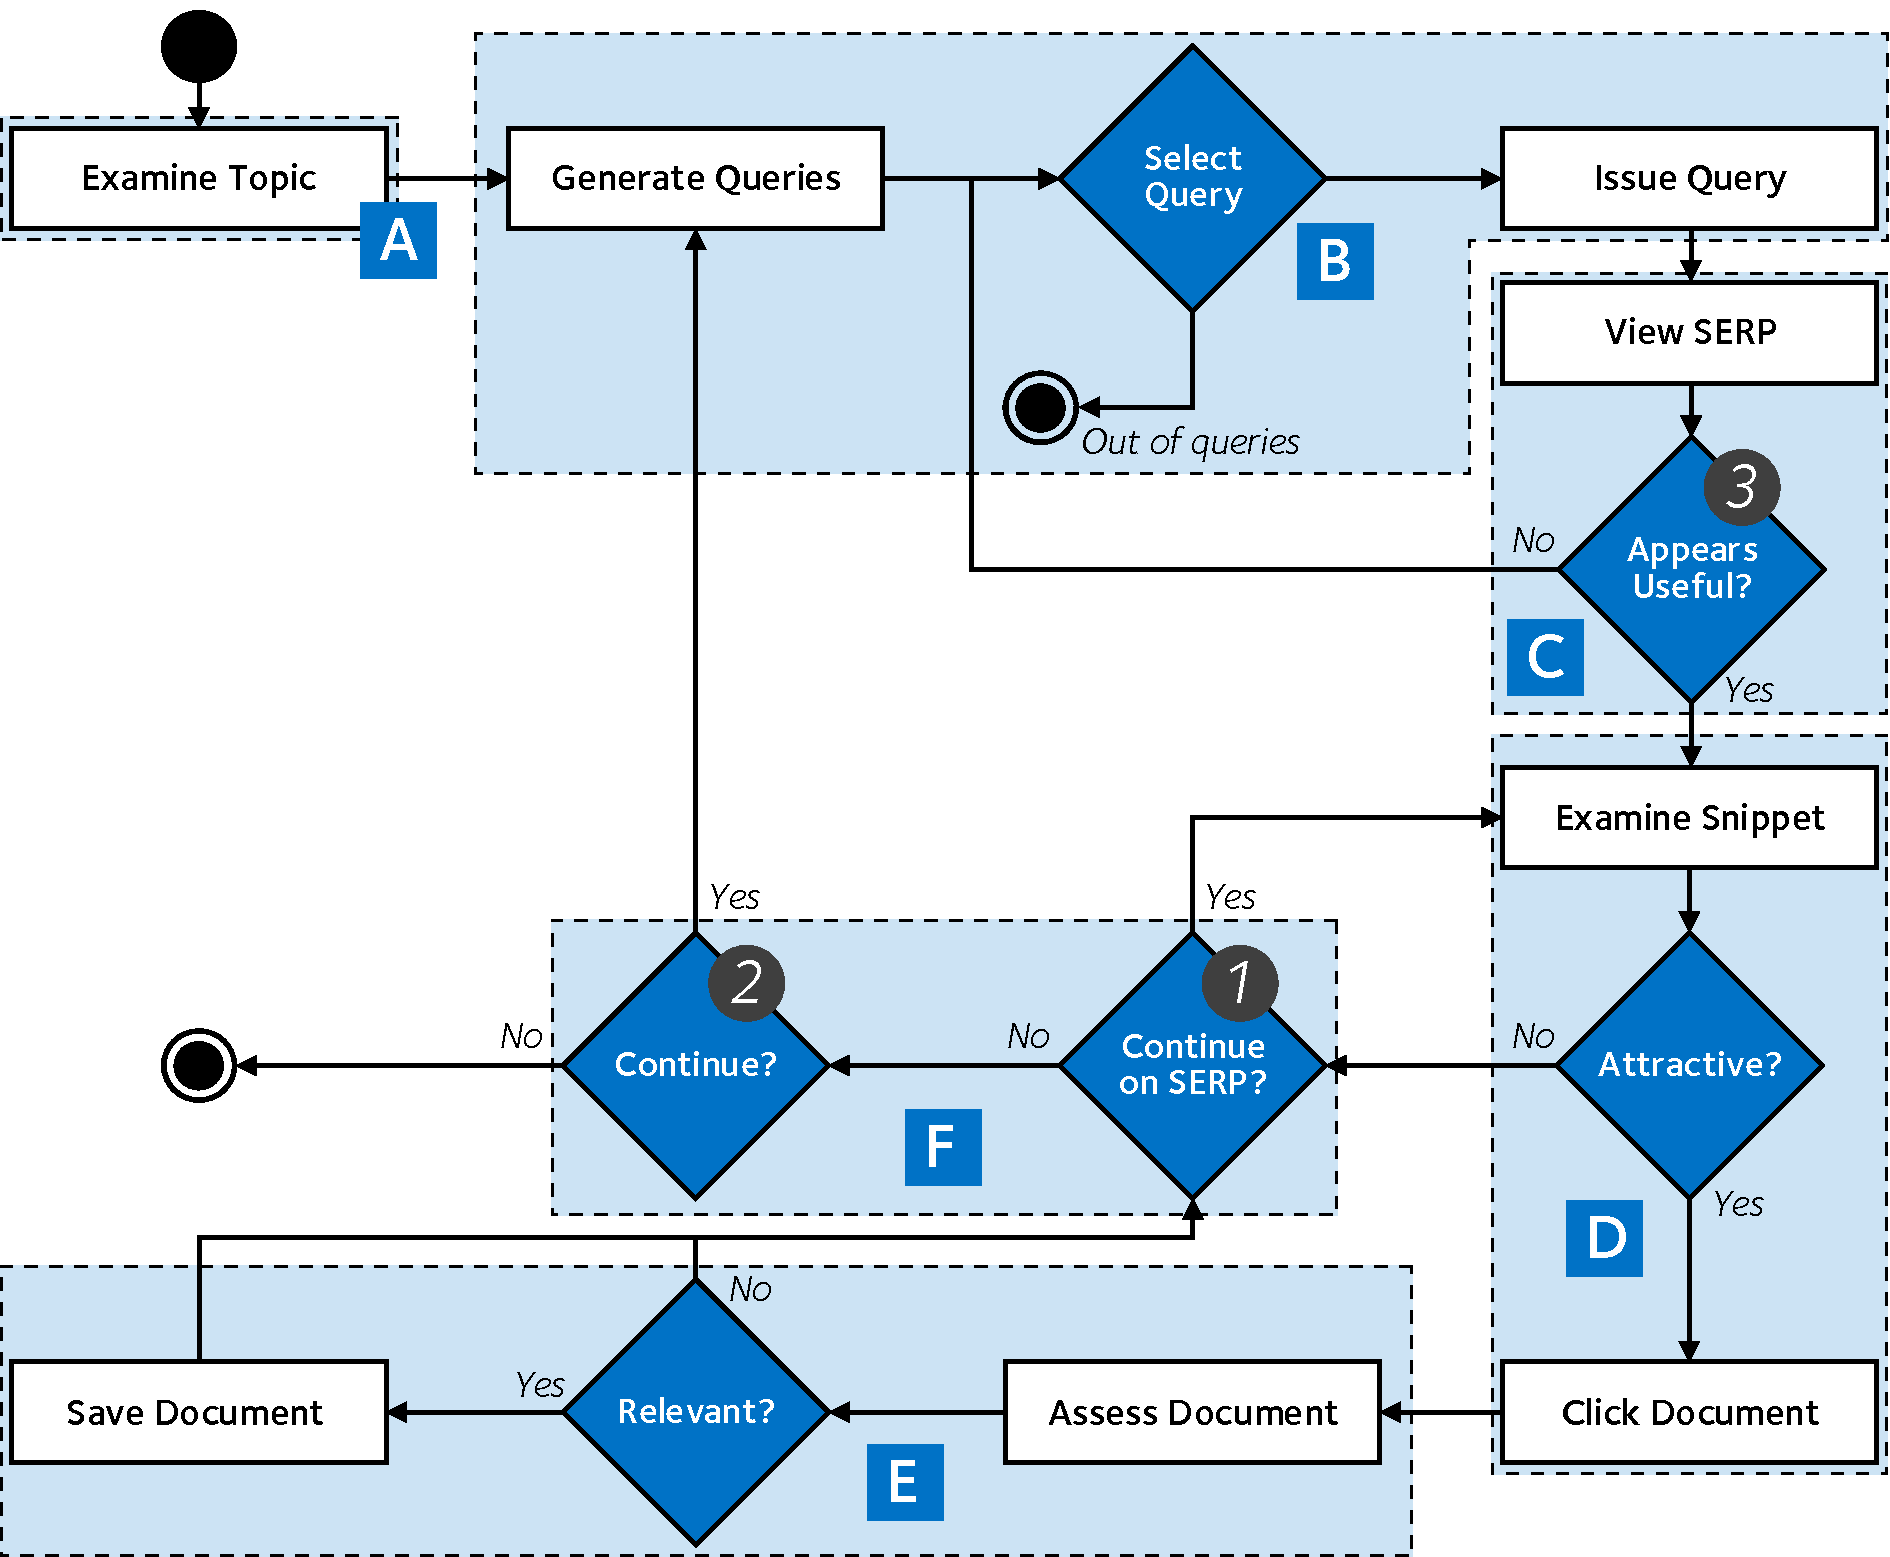
\includegraphics{figures/ch4-csm.pdf}}
    \caption[Flowchart of the~\glsfirst{acr:csm}]{A flowchart of the proposed~\glsfirst{acr:csm}, as used in experimental work discussed later in this thesis. Novel components that the work this thesis provides are highlighted by boxes \blueboxbold{A} and \blueboxbold{B}. The \emph{three} stopping decision points are highlighted with \blueboxbold{1}, \blueboxbold{2} and \blueboxbold{3} (refer to Section~\ref{sec:csm:stopping}). Refer to Section~\ref{sec:csm:csm:flow} for an in-depth explanation of the model.}
    \label{fig:csm}
\end{figure}

\subsection{Model Advancements}\label{sec:csm:csm:advancements}
The~\gls{acr:csm} provides two novel contributions to modelling the information seeking process. The contributions are highlighted as blocks \blueboxbold{A} and \blueboxbold{B} in the~\gls{acr:csm} flowchart provided in Figure~\ref{fig:csm}, and concerns:

\begin{itemize}
    \item[\blueboxbold{A}]{the advancement of modelling the \blueboxbold{querying} aspects of the searcher model; and}
    \item[\blueboxbold{B}]{the introduction of a \blueboxbold{third stopping decision} point concerning the \emph{overall impression} attained of a~\gls{acr:serp} by the searcher.}
\end{itemize}

In the remainder of this section, we discuss these two developments in more detail. While the querying advancements highlighted in block \blueboxbold{A} are novel and intuitive, they are not the core focus of this thesis -- the work detailed in block \blueboxbold{B} is of high relevance, and thus our discussion will be more in depth.

\subsubsection{Modelling the Querying Process}
\begin{publications_box}{Associated Publication}
Work on this advancement of the~\gls{acr:csm} can be found in the following publication.
\vspace*{-2mm}
\begin{itemize}
    \item{\bibentry{maxwell2016agents}}
\end{itemize}
\end{publications_box}

With a search session an inherently interactive process~\citep{ingwersen2005theturn}, a searcher is able to \emph{learn} and develop their mental model of the given information need as they examine information presented to them. As such, during a search task, a searcher may decide to reformulate their query as they obtain a better appreciation of the topic, and are able to formulate a better query, perhaps with descriptive key terms.

As such, the~\gls{acr:csm} provides the mechanism for a searcher subscribing to such a model to update the list of potential queries that could be issued once he or she has finished examining a set of results from the previous~\gls{acr:serp} (labelled as \blueboxbold{Generate Queries} in Figure~\ref{fig:csm}). This is in direct contrast to prior models of search, where queries were selected from a list generated at the start of the search session. This improvement in the modelling process permits a better representation of a searcher's so-called \emph{dynamic information needs}~\citep{borlund2003iir_model}.~\cite{maxwell2016agents} provides an in-depth discussion on this issue.

Once an updated list of queries has been generated, a searcher subscribing to the~\gls{acr:csm} will then make a decision as to \emph{what} query they should issue to the underlying search engine (labelled \blueboxbold{Select Query} in Figure~\ref{fig:csm}). Of course, at this point, a searcher may have exhausted all possible queries, and this is would therefore be a natural stopping point for the searcher. However, as previously discussed, we do not examine this particular component of the~\ref{fig:csm} in any great depth; we do however utilise \emph{querying strategies} that have been previously employed in the literature. Refer to \todo{Section~\ref{}} for more information on these strategies.


\subsubsection{\gls{acr:serp} Level Stopping}
\begin{publications_box}{Associated Publication}
Work on this advancement of the~\gls{acr:csm} can be found in the following publication.
\vspace*{-2mm}
\begin{itemize}
    \item{\bibentry{maxwell2018serp}}
\end{itemize}
\end{publications_box}

As previously mentioned in this section, the second major development, highlighted as block \blueboxbold{B} in Figure~\ref{fig:csm}, is the inclusion of an additional, third stopping decision point. This stopping decision point complements the two established stopping decision points, as discussed in Section~\ref{sec:stopping_background:models:conceptual:simple}.

As outlined by~\cite{maxwell2018serp}, this additional stopping decision point is motivated by the idea of the \emph{information scent} present on a given~\gls{acr:serp}. This was briefly discussed in Sections~\ref{sec:stopping_background:user_studies:understanding} and~\ref{sec:stopping_background:models:theoretical:ift}, and in these sections we highlighted the concept of \emph{proximal cues} providing insights into whether the presented page will yield information that will aid the searcher in satisfying their underlying information need. This has been previously demonstrated in prior studies~\citep{wu2014information_scent, ong2017scent_behaviour, maxwell2017snippets}. By operationalising the notion of information scent as the perceived performance of a given~\gls{acr:serp}, we argue that incorporating this additional activity and stopping decision point allows a searcher to obtain an \emph{impression} of the~\gls{acr:serp} before deciding to \emph{enter} the~\gls{acr:serp} and examine content in detail, or \emph{abandon} the~\gls{acr:serp} and move to the next activity. In other words, when a poor query is issued, the searcher will not expend effort examining content which will have a high probability of not being relevant to their information need. The notion of forming an impression is similar to the summary impressions formed by searchers subscribing to the model defined by~\cite{thomas2014modelling_behaviour}, as detailed in Section~\ref{sec:stopping_background:models:conceptual:simple}. However, in this model, the searcher does not form an overview of the~\gls{acr:serp}, but rather an impression of each summary. This allows him or her to then deduce whether it is enticing enough to examine in more detail.

This is analogous to the well-studied phenomenon of \emph{\gls{acr:serp} abandonment} in which limited interaction occurs with the searcher. This has been typically assumed to provide an indication of the searcher's \emph{dissatisfaction} with the presented results~\citep{dassarma2008serp_abandonment, chuklin2012serp_abandonment}. Thus, we provide, to the best of our knowledge, a model of the search process incorporating a path for a searcher to abandon a~\gls{acr:serp} that appears to be of poor quality (or a \emph{low scent}).

\subsection{Model Flow}\label{sec:csm:csm:flow}
With the underlying assumptions and developments of the~\gls{acr:csm} now outlined, we next provide a high-level description of the various stages of the model. The~\gls{acr:csm} is illustrated as a flowchart in Figure~\ref{fig:csm} on page~\pageref{fig:csm}. Here, the model is described, with an explanation of the different processes involved, and the associated stopping decision points.

When subscribing to the~\gls{acr:csm}, a searcher, once he or she has attained a form of information need, will begin by performing an \blueboxbold{examination of the topic}. This is typically considered to be provided by an experimenter in the form of a \emph{TREC topic}, where a searcher will be provided with a predefined \emph{topic description} of what will constitute as a relevant document (refer to Section~\ref{sec:csm:methodology:collection} for examples). The searcher will then begin to formulate an initial mental model of the topic, identifying key terms and phrases that could be potentially used to translate this information need into a query formulation~\citep{borlund2003iir_model}.

Once a model of the information need has been established, the searcher will then move onto the \blueboxbold{query generation}, \blueboxbold{query selection} and \blueboxbold{query issuance} stages. At this point, the searcher will employ some form of \emph{querying strategy} in order to formulate one or more queries from the underlying model of the information need, and then make a decision, \emph{selecting} one of the candidate queries to take forward and issue to the underlying search engine. As previously discussed, if all candidate queries have been exhausted, the searcher will then stop their search session at this point.

Once a query has been submitted the search engine, the searcher is then presented with the~\gls{acr:serp}. From here, the searcher is able to \blueboxbold{view the~\gls{acr:serp}} -- that is, obtain an \emph{initial impression} from examining the proximal cues presented to him or her. If the~\gls{acr:serp} does not appear to \emph{look good,} or offers a poor information scent, the searcher will abandon the~\gls{acr:serp} and proceed to then issue a further query from the list of candidate queries discussed previously.

If the~\gls{acr:serp} however appears to offer a high information scent, the searcher will then proceed to \blueboxbold{enter the~\gls{acr:serp}}. From here, individual \blueboxbold{snippets will be examined} in detail. As per the assumptions listed above, these are examined in a linear fashion. For each snippet, a judgement is made as to whether the searcher considers it to be sufficiently \blueboxbold{attractive} to click. If deemed sufficiently attractive, the link is clicked, and the searcher is then presented with the \blueboxbold{document} examined in full for an \blueboxbold{assessment}. Once complete, the searcher then makes a further decision with regards to the \blueboxbold{relevancy} of the document to the given information need (or topic, using~\gls{acr:trec} terminology). If deemed relevant, the document is then \blueboxbold{marked} as such, providing a simplistic means for determining what documents have been considered relevant and those that weren't -- refer to Section~\ref{sec:ir_background:user:evaluation:interactive_pr}.

Once the searcher has marked a document as relevant, he or she is returned to the~\gls{acr:serp}. At this point, the searcher must make a decision: \emph{should I continue to examine snippets on this current~\gls{acr:serp}?} This point is also reached by the searcher if he or she judges a snippet to have insufficient attractiveness to pursue further. If the answer is \emph{yes,} the next snippet is examined -- if the answer is \emph{no,} the searcher must then make a further decision. \emph{Given my overall search goals, have I met them? Should I continue my search session?} Search goals will vary between task type -- for ad-hoc retrieval, searchers will often attempt to find a predetermined number of relevant documents before a time limit expires. If the criteria have or criterion has not been met, the searcher will continue his or her search session by jumping back to the near start of the process, and undertake \blueboxbold{query generation} once more. If the stopping criteria have or criterion has been met, then the searcher will then abandon the search session, hopefully satisfied with what he or she has found.

Note that at each process -- whether it be issuing a query or examining a document for relevance -- a searcher will pay some form of \blueboxbold{cost} for the effort that they need to expend performing the aforementioned activity. All of the different components of the~\gls{acr:csm} -- whether they are activities or decision points -- can be instantiated in a number of different ways. For example, stopping strategies that we discuss below in Section~\ref{sec:csm:stopping} can be used to instantiate the different stopping decision points within the model. \todo{What about other bits?}

\subsection{Stopping Decision Points}\label{sec:csm:csm:stopping}
Of central focus to the work in this thesis are the \emph{stopping decision points} of the~\gls{acr:csm}. As previously discussed, the~\gls{acr:csm} contains an additional, third stopping decision point. This is in combination with the two established stopping decision points, as previously highlighted in Section~\ref{sec:stopping_background:models:conceptual:simple} on page~\pageref{sec:stopping_background:models:conceptual:simple}.

The three stopping decision points that the~\gls{acr:csm} considers are listed below. While these are explained in Section~\ref{sec:csm:csm:flow}, it is nevertheless good practice to enumerate them.

\begin{itemize}
    
    \item{\blueboxbold{\gls{acr:serp} Level Stopping} considers the point at which a searcher can abandon a~\gls{acr:serp} after attaining an \emph{initial impression} of the presented~\gls{acr:serp}, thus saving a searcher from examining summaries in depth if the~\gls{acr:serp} appears to be of poor quality.}
    
    \item{\blueboxbold{Snippet Level Stopping} As previously mentioned, this is sometimes labelled as \emph{query level stopping} in the literature. We name this decision point snippet level stopping to remove any ambiguity between~\gls{acr:serp} level stopping and this point. Snippet level stopping considers the depth to which a searcher will traverse a list of results, before deciding to stop their examination.}
    
    \item{\blueboxbold{Session Level Stopping} Finally, session level stopping concerns the notion of when a searcher will decide to terminate their search session altogether. This could be constrained by time limits, or some predetermined notion of how many relevant items they have found.}
    
\end{itemize}

Figure~\ref{fig:csm} on page~\pageref{fig:csm} also provides a visual illustration of the stopping decision points within the wider~\gls{acr:csm} flowchart. Decision points \blueboxbold{1}, \blueboxbold{2} and \blueboxbold{3} represent snippet level stopping, session level stopping and~\gls{acr:serp} level stopping respectively.

How these stopping decision points are operationalised is dependent upon a variety of different factors. For example, the task type is highly likely to influence the overall session stopping strategy that is employed. The literature, as overviewed in Section~\ref{sec:stopping_background:heuristics} provides a number of heuristics to potentially operationalise stopping. These are primarily geared towards the concept of snippet level stopping.

\subsection{Clarifications and Assumptions}\label{sec:csm:csm:assumptions}
As with any model of a real-world phenomenon, the~\gls{acr:csm} also makes a number of key assumptions. Along with clarifications of the model, we list and detail these assumptions below.

\noindent
\blueboxbold{Considering Ad-Hoc Retrieval} The~\gls{acr:csm} considers \emph{ad-hoc retrieval,} a type of search task previously discussed earlier in Section~\ref{sec:ir_background:basics:cranfield:trec}.\footnote{This clarification is included at the request of Distinguished Professor Nicholas Belkin (Rutgers University, NJ, USA), who discussed that the task type the~\gls{acr:csm} models should be clearly defined. This was done at the first \emph{ACM CHIIR} Doctoral Consortium in Chapel Hill, NC, USA -- refer to~\cite{maxwell2016dc} for the associated publication.} Of course, many other different types of search task exist, such as, for example, navigational and patent searching. Ad-hoc retrieval is foundational to many areas of~\gls{acr:ir}\footnote{Referring to \emph{Microsoft} Senior Applied Scientist Peter Bailey's \emph{SIGIR} paper writing tips (available at~\url{https://www.microsoft.com/en-us/research/people/pbailey/} -- last accessed May 1\textsuperscript{st}, 2018), \emph{``there is more to life than ad-hoc''} (tip 10). We agree with this statement, but also argue in the main narrative that the similarities between ad-hoc and other search tasks are similar in nature, making it a sensible choice to consider.} -- but the similarities between ad-hoc and other types of search task provide motivation for selecting such a task to model.

Take, for example, a navigational task. A searcher, wishing to find the electronic commerce site \emph{Amazon}, may issue a query to a commercial web search engine. The query, \texttt{amazon}, yields a series of results presented to him or her on a~\gls{acr:serp}. Typically, if the intent is correctly understood by the search engine, the first result in the verticals links the searcher to Amazon, satisfying his or her information need. This process is largely the same of the~\gls{acr:csm}, as illustrated in Figure~\ref{fig:csm}. Unlike the~\gls{acr:csm} however, the searcher will not complete later stages of the model, such as marking the identified document as relevant -- the searcher will simply abandon the search session.

The argument for using ad-hoc retrieval as the underpinning of the~\gls{acr:csm} is therefore simple. By modelling ad-hoc retrieval, this essentially guarantees that the entire search process -- from query formulation to identifying relevant documents -- is repeated a number of times. As we are modelling the search process in its entirety -- not individual components in isolation -- this makes ad-hoc retrieval a sensible choice.

\noindent
\blueboxbold{Choosing a Search Engine} A searcher, when subscribing to the~\gls{acr:csm}, is assumed to have already undertaken the necessary steps in selecting the search engine most likely to satisfy his or her information need. This is important to clarify, as certain models of information seeking proposed in the literature -- such as the model proposed by~\cite{thomas2014modelling_behaviour} -- include the notion of selecting a search engine within the wider information seeking model. Of course, this is an important step -- selecting a patent search engine\footnote{As opposed to general purpose, commercial web search engines such as \emph{Google} or \emph{Bing,} agencies such as the European Patent Office provide bespoke patent search engines -- refer to \url{https://worldwide.espacenet.com/} for an example (last accessed May 1\textsuperscript{st}, 2018).} for a patent search task would be a prudent choice. We however consider this step superfluous to the requirements of the~\gls{acr:csm} -- the model purely considers the interactions between the user and the search engine, not decisions made before or after.

\noindent
\blueboxbold{Bad and Good~\gls{acr:serp} Abandonment} When considering whether the~\gls{acr:serp} should be abandoned (via the new stopping decision point, summarised in Section~\ref{sec:csm:csm:stopping}), we assume that this is under the pretence of \blueboxbold{bad abandonment} (i.e. a dissatisfaction of the presented results). This is in contrast to the notion of \emph{good abandonment}~\citep{khabsa2016good_abandonment}, which we do not consider in the presented~\gls{acr:csm}. However, future refinement of the model may lead to the ability for the~\gls{acr:csm} to discern between the two -- refer to Figure~\ref{fig:csm_bad_good} for a potential solution to this issue. Indeed, this may be more applicable in future research -- good abandonment is typically prevalent in contemporary~\gls{acr:ir} research (especially on small-screen devices such as smartphones). Furthermore, with the addition of contemporary~\gls{acr:serp} components such as the information card~\citep{bota2016information_cards}, certain information needs can be satisfied by examining the~\gls{acr:serp} without needing to click on any results.

\begin{figure}[t!]
    \centering
    \resizebox{1\hsize}{!}{
    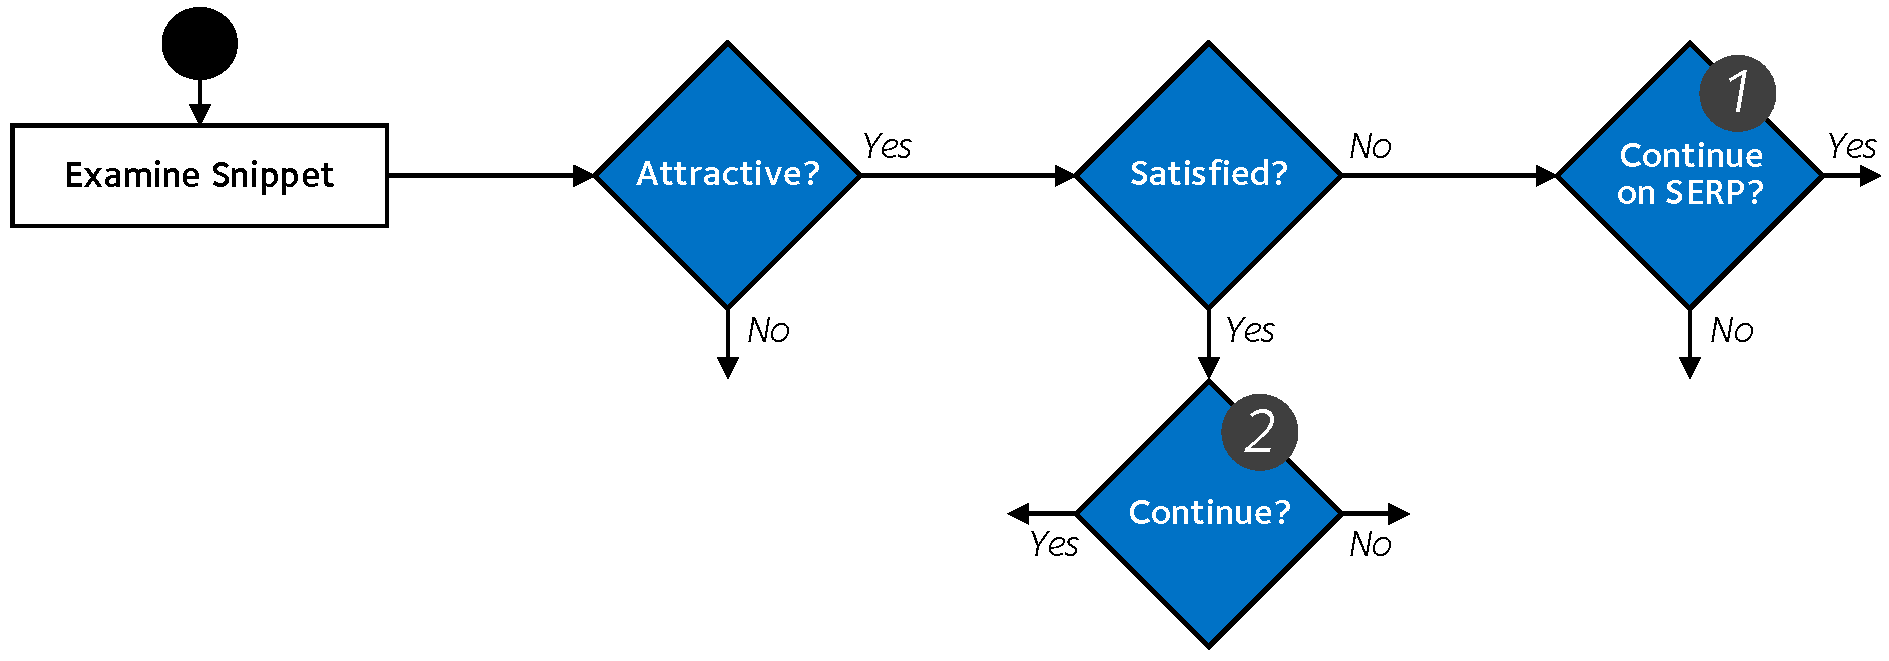
\includegraphics{figures/ch4-good.pdf}}
    \caption[Flowchart considering good abandonment]{A potential solution to also considering good abandonment. After examining a snippet for attractiveness, an additional decision point could allow a searcher to determine that examining the snippet itself satisfies their information need, and thus provide a means by which the searcher could then stop examining results, or stop their search session altogether.}
    \label{fig:csm_bad_good}
\end{figure}

\noindent
\blueboxbold{Simple~\glsplural{acr:serp}} When considering the~\gls{acr:serp} presented to a searcher as a whole, we make three simplifying assumptions within the~\gls{acr:csm}. These are listed and detailed below.

\begin{itemize}
    \item{\blueboxbold{Ten Blue Links} Under the~\gls{acr:csm}, a~\gls{acr:serp} will consist only of one set of \emph{verticals,} i.e. the traditional \emph{ten blue links} that are still present in contemporary~\glsplural{acr:serp}. Of course, we acknowledge that additional components are present in contemporary~\glsplural{acr:serp}, such as multimedia content in federated search~\citep{chen2012federated_search_click_model}.}
    \item{\blueboxbold{Linear Examination Order} Once a searcher has decided to examine a~\gls{acr:serp} in detail, the result summaries presented to the searcher will be examined in the order in which they appear. There is evidence to suggest that real-world searchers examine results from top to bottom, as demonstrated by~\cite{joachims2002click_model} and~\cite{joachims2005click_model}, for example. Click models, such as the \emph{cascade model}~\citep{craswell2008click_models}, have been developed that employ this assumption. Such approaches are subject to \emph{position bias,} where the searcher trusts the results of the retrieval algorithm, assuming that the first result presented in the verticals is the most relevant to their information need.}
    \item{\blueboxbold{No Pagination} The~\gls{acr:csm} also assumes that the~\gls{acr:serp} presented to a searcher is of a single page, and no pagination of results exists. This does simplify the modelling process somewhat, with pagination not considered in prior information seeking models that consider the search session as a whole.}
\end{itemize}

\subsection{Stochastic and Deterministic}
\begin{publications_box}{Associated Publication}
Work discussing the notion of incorporating state and agency into the~\gls{acr:csm} can be found in the following publication.
\vspace*{-2mm}
\begin{itemize}
    \item{\bibentry{maxwell2016agents}}
\end{itemize}
\end{publications_box}

In this section, should I explain the difference between stochastic models of search, and deterministic models of search?
So, in a previous section, we detailed different approaches to simulation.

Stochastic considers a `roll of the dice' to determine whether a searcher will click on a link, for example $P(C)$. And that can be drilled down even more, to consider probability of a click given that it is relevant to some gold standard $P(C|R)$.

Other alternative is to instantiate the model using deterministic components.
So that the searcher is able to deduce, without grounding, what is relevant and not. Dependent upon various components like language models, and is much more complex. This is more in tune with attempting to model the cognitive functions going on inside someone's brain, and is not really the focus of this thesis.

However, we have explored this in detail. In~\cite{maxwell2016agents}, we looked at the notion of developing intelligent search agents with the~\gls{acr:csm}. (Short explanation of paper).

These are dependent upon the state of a user. We argue that even a simple implementation of the CSM itself has some form of state, because it needs to remember things like: what documents it has clicked on, what documents it has marked, and so forth. It needs to keep track of queries it has issued, so it does not issue duplicates. Basic things. In this agency paper, we took it further, so the searcher was able to `learn' and make informed decisions (i.e. training a language model) at each iteration of the search process.

So... in this thesis, we consider only stochastic models of search, where the simulations are grounded with some prior probabilities extracted from interaction data. The approach is discussed more in Section~\ref{sec:csm:methodology}.


\section{Operationalised Stopping Strategies}\label{sec:csm:stopping}
In Section~\ref{sec:stopping_background:heuristics}, we discussed a number of different \emph{stopping heuristics} that have been previously defined in the literature. A majority of these heuristics were derived from the concept of \emph{satiation}~\citep{simon1955satiation} -- that is, the searcher abandons their search when they feel satisfied with what they have found. These heuristics were conceptual in nature, being derived from a number of underlying theories and assumptions.

In this section, we take a number of these stopping heuristics forward to produce a number of different~\glsplural{glos:stopping_strategy}. These strategies are operationalised versions of the corresponding heuristics, which mean we can subsequently implement and test them. The stopping strategies are enumerated, and split into five main categories, as listed below:

\begin{itemize}
    \item{a baseline, \blueboxbold{fixed depth} stopping strategy;}
    \item{a stopping strategy based upon the \blueboxbold{frustration} stopping heuristic;}
    \item{\blueboxbold{satisfaction} based stopping strategies;}
    \item{stopping strategies based upon the \blueboxbold{difference} threshold stopping heuristic;}
    \item{several stopping strategies based upon~\blueboxbold{\gls{acr:ift}}; and}
    \item{two stopping strategies based upon established~\gls{acr:ir} evaluation measures.}
\end{itemize}

Although each of these stopping strategies could in theory be applied to any of the three stopping decision points summarised in Section~\ref{sec:csm:csm:stopping}, we consider them only from a snippet level in this thesis. This does not mean to say we do not explore the additional two stopping decision points -- Chapter~\ref{chap:serp} explores the~\gls{acr:serp} level stopping decision point, and Chapter~\ref{chap:diversity} considers the session level stopping decision point.

In addition to this, not all stopping heuristics outlined in Section~\ref{sec:stopping_background:heuristics} are considered. This is because several of the stopping heuristics are not trivial to implement, and would require considerable effort to model effectively. Furthermore, a number of these heuristics do not necessarily comply with the search task we will be simulating -- the mental list heuristic may not be directly applicable to ad-hoc retrieval, for example.

\todo{The following stopping strategies have been catalogued in Section~\ref{sec:stopping_background:heuristics}. It should be noted that we have not selected rules which are based upon satisfaction or satiation because the task we are investigating is ad-hoc topic retrieval, where the goal is to find as many relevant documents as possible in a given period of time. The satisfaction/satiation rules therefore do not seem particularly applicable in this context. Furthermore, rules such as the mental list rule seem to be more topic specific, requiring a searcher to know in advance all the criteria that they need to check off in their head \emph{a priori}. However, these criteria are largely unknown in ad-hoc circumstances.}

\noindent\blueboxbold{A Note on Usefulness} In this section, we refer to the concept of a result summary being \emph{useful} and \emph{unhelpful}. By this, we mean that a summary appears to be of use for a searcher to satisfy his or her information need. In the context of simulation, this notion of relevance does not necessarily correspond to the judgement made in a gold standard that is being compared to: the notion of usefulness in this context represents the decisions that are taken by a searcher as to what constitutes a useful or unhelpful document/result summary.

\begin{publications_box}{Associated Publications}
A number of the stopping strategies listed below have been previously defined in the following publications.
\vspace*{-2mm}
\begin{itemize}
    \item{\bibentry{maxwell2015initial_stopping}}
    \item{\bibentry{maxwell2015stopping_strategies}}
\end{itemize}
\end{publications_box}

\subsection{Fixed Depth}
The fixed depth stopping strategy is based upon an assumption held across many of the models and measures that are widely used throughout the~\gls{acr:ir} community. This assumption is that a searcher, when examining a list of ranked results for their query, will browse to a \emph{fixed depth} before stopping -- the roots of which can be traced back to the Cranfield Paradigm as discussed in Section~\ref{chap:intro}. Examples of use include the basic stopping model encoded within~\gls{acr:patk}. The assumption is also widely used in the simulation of interaction. For example,~\cite{azzopardi2011economics} conducted a large-scale simulated analysis, where simulated users examined content to depths ranging from $5$ to $1,000$ ($1,000$ is typically assumed in TREC style experimentation, where a single query is issued). Given the wide use of this fixed depth approach in historical and contemporary~\gls{acr:ir} research, we consider this stopping strategy as the baseline approach to which we will be comparing the more advanced, \emph{adaptive} stopping strategies.

\begin{itemize}
    
    \item[]{\blueboxbold{SS1}} Using this stopping strategy, a searcher will stop once they have observed $x_1$ result summaries (i.e. \blueboxbold{SS1} @ $x_1$), regardless of their relevance to the given topic.
    
\end{itemize}

\begin{figure}[t!]
    \centering
    \resizebox{1\hsize}{!}{
    
\includegraphics{figures/ch4-ss1.pdf}}
    \caption[Examples of the fixed depth stopping strategy, \blueboxbold{SS1}]{An example of the fixed depth stopping strategy, stylised in this thesis as \blueboxbold{SS1}. Here, a searcher has an information need for the conference \emph{CIKM 2015} in Melbourne, Australia. The left example shows the top five results for poor performing query query, with few useful results (denoted by {\color{dmax_red}crosses}); conversely, the right shows results for a query performing well, with many useful results (denoted by {\color{dmax_green}ticks}). With \blueboxbold{SS1} @4, the searcher will stop at a depth of 4, regardless of the usefulness of the content provided.}
    \label{fig:ss1}
\end{figure}

Given the description of the stopping strategy above, we note that the fixed depth approach is na\"{i}ve in the sense that documents up to rank $x_1$ are useful to the searcher's given information need. On average, such a rule does make sense, but when individual result lists are considered, the approach would not be considered to be a sensible strategy to follow.

Despite the na\"{i}evty of the approach, the other main drawback of such an approach is exposed when a searcher complying with such a strategy issues a poor performing query. This is demonstrated in Figure~\ref{fig:ss1}, with two~\glsplural{acr:serp} presented side by side. Given a searcher's desire to find pages that provide information regarding \emph{CIKM 2015}\footnote{CIKM 2015 was a conference held in Melbourne, Australia, in October 2015. The paper that initially proposed many of these stopping strategies~\cite{maxwell2015stopping_strategies} was indeed presented at this conference.}, two queries are issued: the query on the left yielding poorer results than the query on the right, as denoted by the ticks and crosses, for useful and unhelpful result summaries, respectively. With \blueboxbold{SS1} @4 set, four result summaries are always examined before stopping, regardless of their perceived usefulness. As a result of this, na\"{i}vely examining four documents for the query on the left is by and large a waste of the searcher's time.

\subsubsection{Considering Searcher Frustration and Satisfaction}
In this section, we propose three further stopping strategies, based upon a searcher's tolerance to non-relevance (frustration) and a simple goal-based strategy (satisfaction).

\subsubsection{Searcher Frustration}
he second category of stopping strategies that we propose in this thesis are those that consider a searcher's \emph{tolerance to non-relevance}. Given a set of result summaries presented on a~\gls{acr:serp}, how many would a searcher be prepared to judge to be of no use before they become frustrated, and subsequently abandon their query?

As detailed in Section~\ref{sec:stopping_background:heuristics}, a number of researchers have proposed stopping heuristics that consider non-usefulness (or \emph{non-relevance}, as defined in the literature). The rule intrinsically makes sense for exhaustive searches~\cite{kraft1979stopping_rules}. As an example, when tasked to find as many documents as possible related to different species of animals that are endangered, becoming disgusted with the presented~\gls{acr:serp} when a lack of new species are shown would be a suitable point at which to break and reformulate a new query, or abandon the search session altogether.

From the heuristics defined by~\citealt{cooper1973retrieval_effectiveness_ii} and~\citealt{kraft1979stopping_rules}, we propose two variants of the disgust rules, \blueboxbold{SS2} and \blueboxbold{SS3}.

\begin{itemize}
    
    \item[]{\blueboxbold{SS2}} Under this stopping strategy, the searcher will stop once they have observed $x_2$ unhelpful result summaries. If a result summary has been previously seen in the search session and was considered non-relevant, it is included in the count.
    
    \item[]{\blueboxbold{SS3}} Similar to the stopping strategy defined above above, a searcher employing this stopping strategy will stop once they have observed $x_3$ unhelpful result summaries \emph{in a row (contiguously)}. Previously observed unhelpful result summaries within the search session are included in the count.
    
\end{itemize}

\begin{figure}[t!]
    \centering
    \resizebox{1\hsize}{!}{
    
\includegraphics{figures/ch4-ss23.pdf}}
    \caption[Examples of frustration rules \blueboxbold{SS2} and \blueboxbold{SS3}]{An example of the two frustration rules, \blueboxbold{SS2} (left) and \blueboxbold{SS3} (right), both using a parameter of 3 unhelpful result summaries, and under the same query and results. Given that \blueboxbold{SS2} considers the \textbf{total} number of result summaries judged to be unhelpful, a searcher employing this stopping strategy would stop at rank 5 in the example above. Considering a set of contiguous unhelpful summaries, a searcher using \blueboxbold{SS3} would stop at rank 7.}
    \label{fig:ss23}
\end{figure}

As mentioned previously, these two stopping strategies are the first that we enumerate where a searcher would begin to \emph{adapt} their interactions with a ranked list of results, depending upon the performance of the underlying query that was issued. As such, this behaviour inherently makes these stopping strategies more realistic~\cite{moffat2013users_versus_models}. Figure~\ref{fig:ss23} illustrates this adaption in action, with the same query and associated results. On the left of the figure is an illustration of when a searcher employing \blueboxbold{SS2} would stop, and on the right, an example of \blueboxbold{SS3}. We use $x_2 = x_3 = 3$. Under \blueboxbold{SS2}, a searcher would stop at rank 5, while a searcher would stop at rank 7 when employing \blueboxbold{SS3}.

\cite{cooper1973retrieval_effectiveness_ii} highlights the above as one way of operationalising such a stopping strategy: by providing a pre-determined number of documents to stop at. The other approach, which we do not consider in this thesis, would be to allow a searcher to find a series of documents, then go back and count. Such an approach seems unnatural, with the former approach simulating a form of goal-based task. By varying the number of non-relevant documents to stop at, one will be able to attain a better understanding of how performance and other behaviours differ.

\subsubsection{Goal/Satisfaction Based}
Analogous to the frustration rule are the satiation-based stopping heuristics. Here, rather than focus on the frustration or disgust that a searcher might experience when confronted with unhelpful result summaries, satisfaction based rules -- explained in Section~\ref{sec:stopping_background:heuristics:judgement:satisfaction_frustration} -- consider a searcher encountering a number of \emph{useful} result summaries (or documents) before deciding to stop.

\begin{itemize}
    \item[\blueboxbold{SS4}] A searcher using this stopping strategy will stop examining content after encountering $x_4$ useful result summaries.
\end{itemize}

While demonstrated above in the context of snippet level stopping, such a strategy, depending upon the search task, may not be particularly useful when operationalised at this stopping decision point. For example, consider the scenario where a searcher issues a poor query, yielding next to no summaries deemed to be worthy of further examination. In this scenario, a searcher fully complying with \blueboxbold{SS4} may struggle to find enough documents to reach their goal, and this will waste time examining poor results. Such a stopping strategy may be better suited to an overall search goal (i.e. a session level stopping strategy), and deploying a more suitable stopping strategy for snippet level stopping decisions.


\subsubsection{Combining Frustration and Satisfaction}
Considering satisfaction and frustration based stopping heuristics,~\citealt{kraft1979stopping_rules} also proposed a \emph{combination heuristic} that combined both approaches together. Employing this heuristic, a searcher would stop when they became frustrated, or were satisfied by what they saw -- whatever comes first. As such, we can convert this into a stopping strategy, as described below.

\begin{itemize}
    \item[\blueboxbold{SS5}] A searcher utilising this stopping strategy will employ \blueboxbold{SS2} and \blueboxbold{SS4} to determine when to stop, ceasing their search on the~\gls{acr:serp} for the first stopping strategy whose criterion is met.
\end{itemize}

Note that we consider only a searcher's total tolerance to non-relevance (i.e. \blueboxbold{SS2}), not \blueboxbold{SS3}.


\subsection{Considering the Difference}
\todo{rewrite}
The next two stopping strategies are based upon the difference threshold heuristic. To operationalise this rule, we consider the difference between the text of the current snip- pet and the text of previously examined snippets. Here, the idea is that as simulated searchers examine snippets, they may encounter a snippet that is not sufficiently different from what they already have observed, meaning that they are unlikely to find new information. The searcher therefore stops and issues a new query. From this rule, we devised two separate stopping strategies where we computed the difference based upon term overlap and KL-Divergence scores.

\begin{itemize}
    \item[\blueboxbold{SS6}] This stopping strategy compares the occurrences of terms in a given snippet against all terms in previously examined snippets. The more terms that overlap, the greater the chance that the new snippet does not contain any new information. If $\frac{|s_{curr} \cup s_{prev}|}{|s_{curr}|} > x_6$, the new snippet is considered too similar to previously examined content. The searcher will then move to the next query. Here, $s_{curr}$ denotes the terms of the current snippet, $s_{prev}$ denotes terms from all previously observed snippets, and $x_6$ is the threshold at which the searcher will stop.
\end{itemize}

\begin{itemize}
    \item[\blueboxbold{SS7}] This stopping strategy considers KL-Divergence as a means for comparing a given snippet against previously observed snippets. If the resulting value is less than threshold $x_7$, then the snippet is considered too similar to previously seen content, and the searcher stops, moving to the next query.
\end{itemize}

When implementing \textbf{\emph{SS4}} and \textbf{\emph{SS5}}, we considered the \emph{per-query difference} and the \emph{per-session difference}. For the per-query variant, previously observed text consisted of the first snippet, thus meaning that the simulated searcher always considers at least two snippets before stopping. For the per-session variant, all previously seen snippets over the simulated search session are used. In this paper, we will only report the per-query variants of \textbf{\emph{SS4}} and \textbf{\emph{SS5}}, as both performed somewhat better than their per-session variants in a pilot study. A number of other variants were also considered but not explored, such as using the document and snippet text, and using only text from snippets considered relevant. To compute the KL-Divergence, we used a \emph{Maximum Likelihood Estimate (MLE)} of the term distribution given the new snippet, and all the previously examined snippets. We also explored smoothing the distribution with the probabilities of each collection used. However, this approach was not used; performance was not increased, only complexity.

\subsection{Considering Information Foraging Theory}
We look at IFT now -- so we have the optimal stopping rule, as previously discussed in Section~\ref{} and a number of rules borrowed from ecology that consider the time a searcher will spend examining a \emph{patch} before moving on.

\subsubsection{Optimal Foraging}

\begin{itemize}
    \item[\blueboxbold{SS8}] With this stopping strategy, a searcher is assumed to have some idea of the average rate of gain (denoted as $x_6$). If the rate of gain from the observed documents thus far does not exceed $x_6$, the searcher then stops and proceeds to issue the next query.
\end{itemize}

To determine the rate of gain at the current snippet, we first computed the \emph{Discounted Cumulative Gain (DCG)} $g$ received from the observed documents up to that point in the ranked list at position $i$. We then divided $g$ by the total time taken, i.e. $i*t_d +t_q$, where $i$ represents the rank, $t_d$ is the time taken to examine a document, and $t_q$ is the time taken to issue a query. This estimate is very dependent upon the first document. For example, if the first document is non-relevant, then the gain is zero, and thus the simulated searcher would immediately stop when $x_6>0$. We also included another parameter which specifies how many snippets they should first consider before making their decision based on the rate of gain\footnote{\scriptsize{This parameter was set to 2 for this study - refer to Section~\ref{sec:method:stopping}.}}. This would essentially mean that the simulated searcher would look at $y_6$ snippets/documents, and then decide to continue with the current query.

\subsubsection{Time-Based Strategies}
More directly connected to stopping is the Information Patch Model~\cite{pirolli1999ift} which is derived from Optimal Foraging Theory. The stopping rule from Foraging Theory is based on Charnov's Maximal Marginal Theorem~\cite{charnov1976mvt}, which states that when the rate of gain within the patch falls below the average rate of gain in the environment then the forager will stop (see Figure~\ref{fig:ift_patch}). This lead to the \emph{instantaneous intake} rule, where a forager will leave when their rate of gain falls below a given threshold (refer to Figure~\ref{fig:ift_patch}). However, it is often difficult to operationalize this rule/theorem in practice. Instead several other stopping rules that influence patch leaving decisions have been developed in Foraging Theory ~\citet{stephens1986foraging_theory}, which approximate the theorem. These  include: the \emph{number rule}~\cite{gibbs1958number_rule}, where a forager stops after finding $n$ prey (similar to the satisfaction~\cite{cooper1973retrieval_effectiveness} and satiation rules~\cite{kraft1979stopping_rules}); the \emph{time rule}~\cite{krebs1973time_rule}~\cite{charles1972behaviour}, where a forager stops after $x$ seconds; the \emph{leave after an $x$} rule~\cite{krebs1974leave_after_rule}, where a forager would stop after $x$ seconds of unsuccessfully finding anything. A study of different \emph{patch types} (i.e. where the density of prey varies), was conducted by~\citet{mcnair1982gut_mvt} who found that across different patch types, different stopping rules worked better in different environments~\cite{mcnair1982gut_mvt, green1984oft_stopping, iwasa1981prey_distribution}. Consequently, a combination rule was devised where in a patch that is fruitful early on, a satisfaction/satisficing rule would perform well; otherwise employing the leave after $x$ rule would work best. In this paper, we develop several new stopping strategies based on these rules from Optimal Foraging Theory and also introduce a SERP level stopping decision component that considers the information scent of the page before examining the snippets in detail.

\begin{figure}[t!]
    \centering
    \resizebox{1\hsize}{!}{
    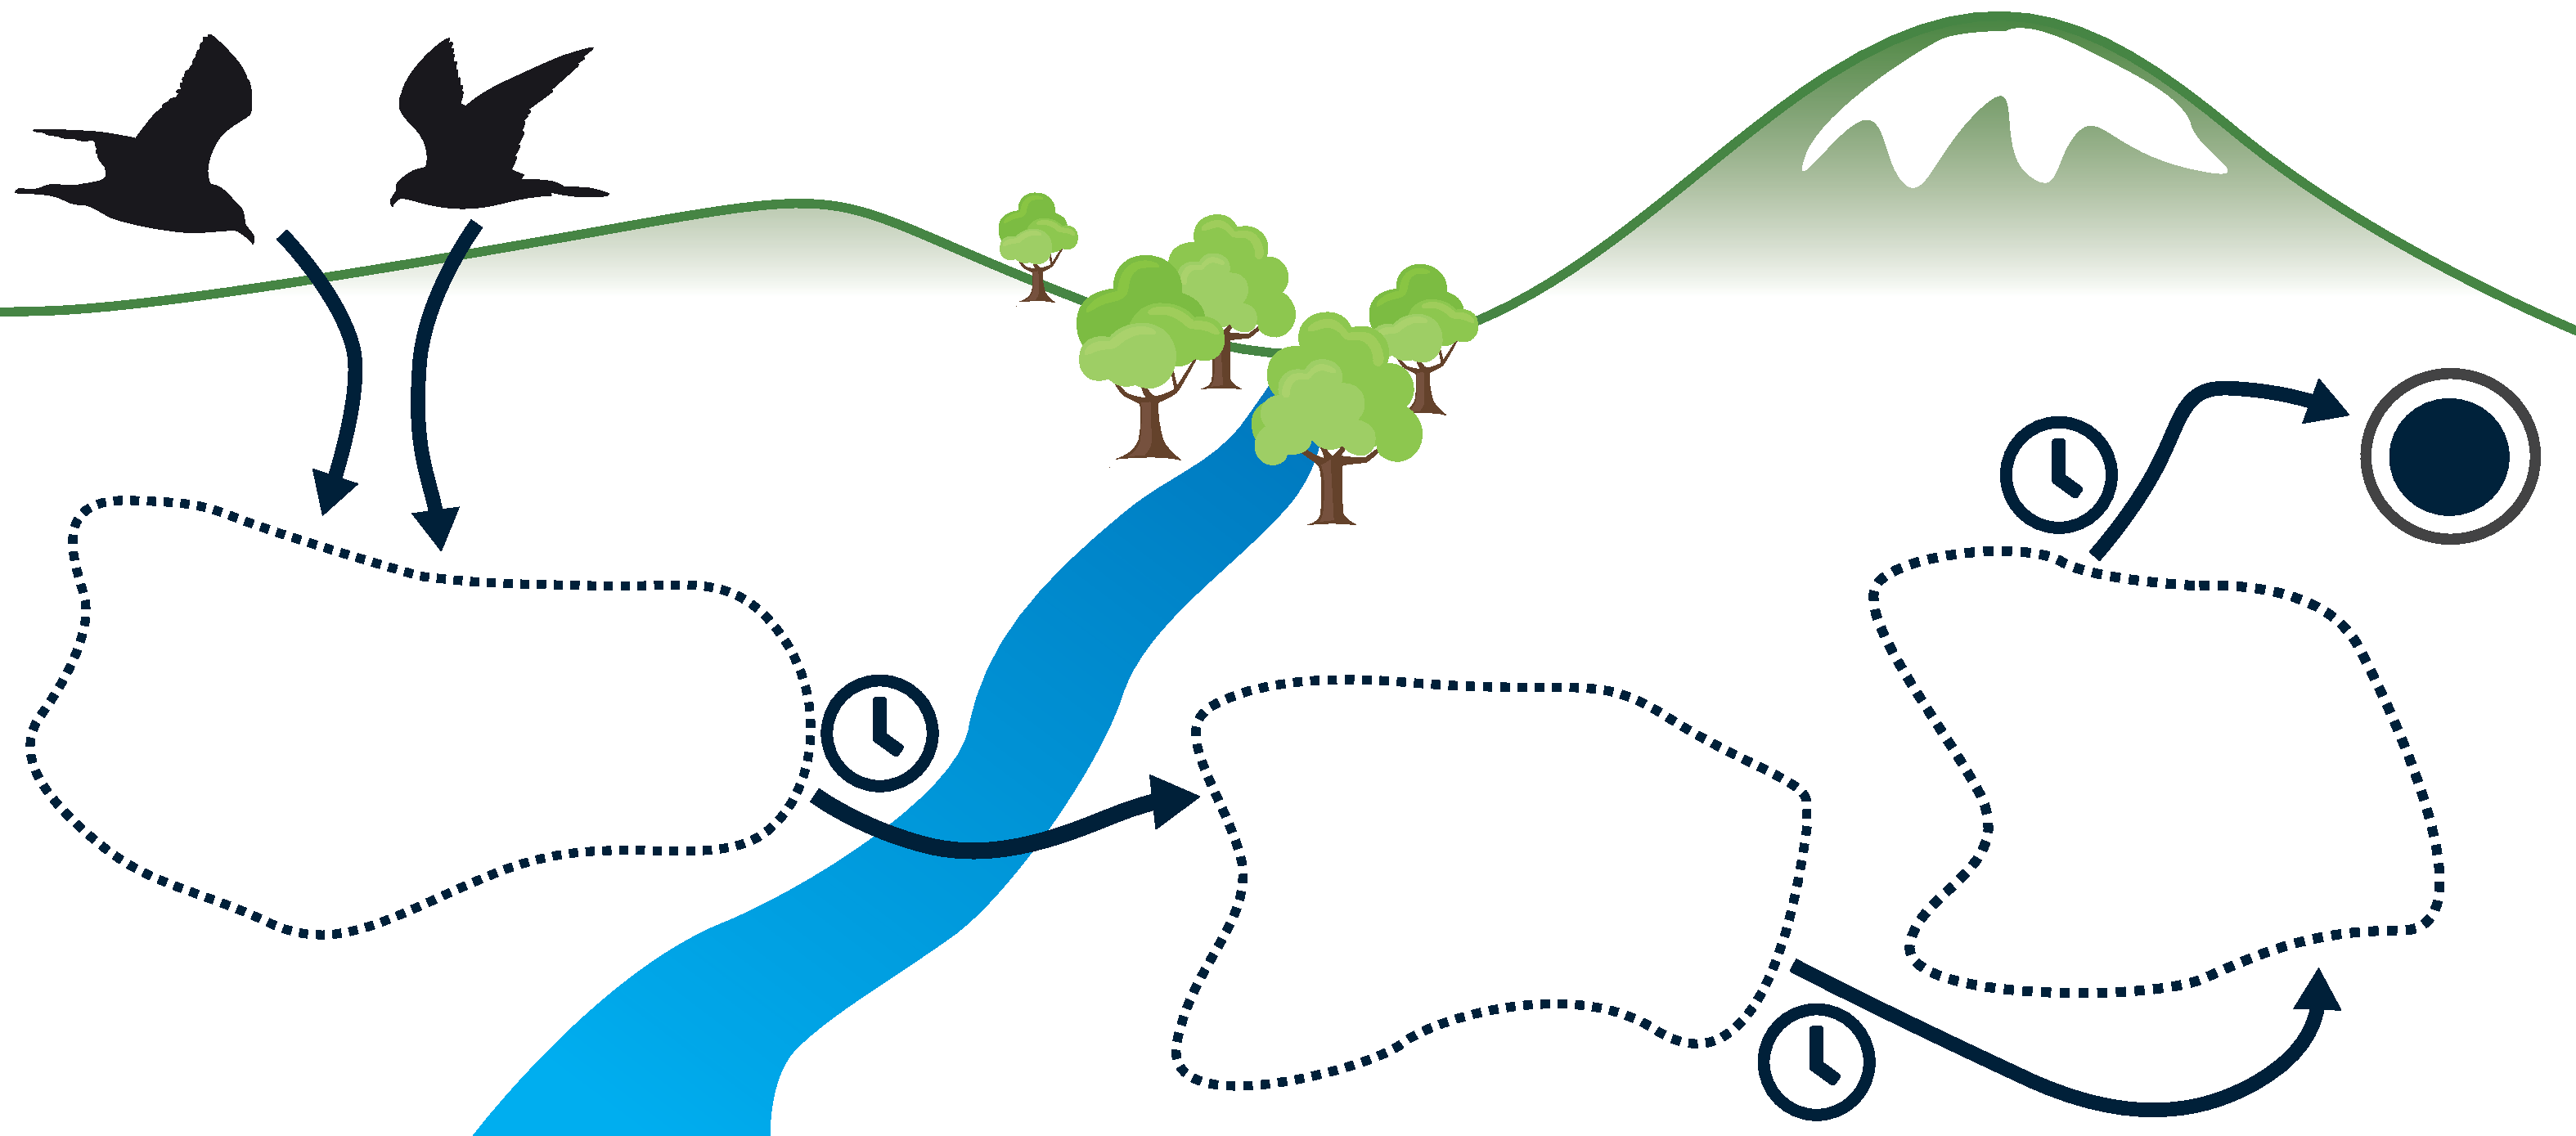
\includegraphics{figures/ch4-gut.pdf}}
    \caption[Give Up Time]{The give up time}
    \label{fig:gut}
\end{figure}

The next two strategies are based on the \emph{time} rule and the \emph{Giving Up} rule~\cite{gibbs1958number_rule}:

\begin{itemize}
    \item[\blueboxbold{SS9}] Employing this stopping strategy, a searcher will leave a SERP after $x_9$ seconds have elapsed from first entering it.
\end{itemize}

\begin{itemize}
    \item[\blueboxbold{SS10}] A searcher employing this strategy will stop after $x_10$ seconds have elapsed since a snippet judged to be relevant was found. If no relevant items have been encountered on the given SERP, then the searcher will stop after $x_9$ seconds have elapsed since arriving at the SERP.
\end{itemize}

These stopping strategies are similar to the frustration based strategies previously proposed (i.e. \textbf{SS2} and \textbf{SS3}) except bound by time~\cite{gibbs1958number_rule}. As mentioned earlier ~\citet{mcnair1982gut_mvt} studied how animals would change their stopping strategies based on their initial evaluation  of the patch, where his suggested combination rule would be as follows.

\begin{itemize}
    \item[\blueboxbold{SS11}] When encountering a SERP expected to yield a high volume of relevant content early on (high scent), the searcher will employ the satisfaction stopping strategy \textbf{SS8S}. If the SERP however yields relevant items over greater depths, or is judged to be of poor quality (low scent), the giving-up stopping strategy, \textbf{SS10G}, is used instead.
\end{itemize}

The combination rule tries to ensure that searcher avoids wasting time on patches with a low yield, but capitalize on patches with a high yield. In the following section, we shall describe the simulated analysis to compare the existing and proposed stopping strategies.

\subsection{\gls{acr:ir} Evaluation Measures}
As previously mentioned most evaluation measures implicitly encode some stopping model (e.g. P$@$10 encodes SS1$@$10). Two measures that have been recently proposed that explicitly encode a stopping model are \textbf{RBP}~\cite{moffat2008rbp} and \textbf{INST}~\cite{bailey2015inst, moffat2015inst}. 
Under \textbf{RBP}, the decision to continue to the next results is based on the patience parameter (e.g. the probability of continuing), while under \textbf{INST} the probability of continuing is based on how many the documents the searcher expects to encounter, how many they have encountered and their current rank - essentially the probability of continuing decreases as they encounter more relevant information, and as they progress further down the ranking.

\begin{itemize}
    \item[\blueboxbold{SS12}] RBP
\end{itemize}

\begin{itemize}
    \item[\blueboxbold{SS13}] INST
\end{itemize}

The satisfaction stopping strategy \textbf{SS8S} was set to consider $1$ to $7$ (hence providing values for $x_8$). A maximum of seven was chosen as this was closest integer to the mean number of documents marked by subjects in the log data. With our \textbf{INST} stopping strategy employing a similar approach, considering the ``number of useful pages that the searcher expects they will need''~\cite{moffat2015inst}, we subsequently set $T$ in INST to the same range. For our other baseline, \textbf{RBP} considers a \emph{patience factor} that influences the depth to which a searcher is prepared to tolerate examining to. Using the log data we estimated the patience of users to be approximately $p=0.9087$. In this study, examined patience from $0.8$ to $0.95$ in steps of $0.05$, and also $0.99$.

\section{General Methodology Overview}\label{sec:csm:methodology}
In Chapters~\ref{chap:snippets} and~\ref{chap:diversity}, we will be exploring how an individual's searching behaviours (particularly their stopping behaviours) vary under differing contexts. This section provides a high level overview of the \emph{general methodology} that we will employ in these two chapters, focusing on four main tasks:

\begin{itemize}
    \item{conducting a \blueboxbold{user study} to examine real-world searcher behaviours;}
    \item{extracting the \blueboxbold{interaction data and performance measures} from the user study;}
    \item{using the aforementioned data to ground a series of \blueboxbold{simulations} that attempt to replicate the user studies; and}
    \item{\blueboxbold{evaluating} the performance of the simulated users, and \blueboxbold{comparing} the simulated user behaviours against those of their real-world counterparts.}
\end{itemize}

We now discuss each of these different tasks in greater depth, highlighting the key decisions and \todo{assumptions} that we have made. Note that this section is directly applicable to contributory Chapters~\ref{chap:snippets} and~\ref{chap:diversity}; Chapter~\ref{chap:serp} provides an in-depth examination on the realism of the~\gls{acr:csm} before we employ it in the following two contributory chapters. Indeed, given that this chapter relies solely on simulations, we follow the approach followed in Section~\ref{chap:csm:method:simulation} and~\ref{chap:csm:method:evaluation}. However, we do ground our experimentation in Chapter~\gls{acr:csm} with user study interaction data from a following chapter.

% Now that we have outlined the~\gls{acr:csm} and the various stopping strategies that we will operationalise, this section provides a high level explanation of the \emph{general methodology} that we will employ in subsequent contributory chapters of this thesis.
%
%
%
% Now that we have outlined the~\gls{acr:csm} and the various stopping strategies that we will operationalise, this section provides a high level explanation of the general methodology of the subsequent contributory chapters. Chapters~\ref{chap:snippets} and~\ref{chap:diversity} will follow this approach, along with the work detailed in Chapter~\ref{chap:serp}.
%
% In essence, the main aim of the following contributory chapters is to examine what happens to a searcher's behaviours (in particular, their stopping behaviours)
%
%
% ground the data
% ground the simulation
% evaluate it later on
% explore influence of these decision points and stopping strategies under different contexts
%
% We want to examine what happens to a searcher's behaviour when different stopping rules are employed under certain contexts.
% How can we do this? Here, we provide a broad overview of the methodology that was employed in the later chapters of this thesis. Broadly split across two main sections.

\subsection{Test Collection, Topics and Search Engine}\label{sec:csm:methodology:collection}
Central to any~\gls{acr:ir} experiment is a corpus of documents (refer to Section~\ref{sec:ir_background:basics:indexing}) with which subjects participating in the experiment can issue queries against. In conjunction with the document corpus, a number of topics are also used to provide simulated information needs.

For the contributory chapters of this thesis, all work detailed uses the TREC AQUAINT corpus, consisting of over one million news articles from the period ranging 1996 to 2000. All of the news articles were collected from three newswires, namely: the \emph{Associated Press (AP);} the \emph{New York Times (NYT);} and \emph{Xinhua}. More contemporary collections could have been used; the reasons for selecting an older were twofold: \emph{(i)} using such a collection enabled us to easily evaluate the performance of subjects; and \emph{(ii)} employing the AQUAINT corpus provides continuity with a prior line of research using this collection, as shown by~\cite{azzopardi2013query_cost}, for example.

Five topics were also selected from the 50 provided in the \emph{TREC 2005 Robust Track,} as outlined by~\cite{voorhees2006trec_robust}. These topics were selected based upon evidence from a previous user study (of similar nature) conducted by~\cite{kelly2015serp_size}. Evidence showed that the topics offered similar levels of difficulty. The five topics, along with a short description of what constitutes a relevant document, are listed below. These summaries are derived from the TREC topic descriptions that are provided as part of the TREC 2005 Robust Track -- Figure~\ref{fig:topics} illustrates three examples of topic descriptions.

\begin{figure}[t!]
    \centering
    \resizebox{1\hsize}{!}{
    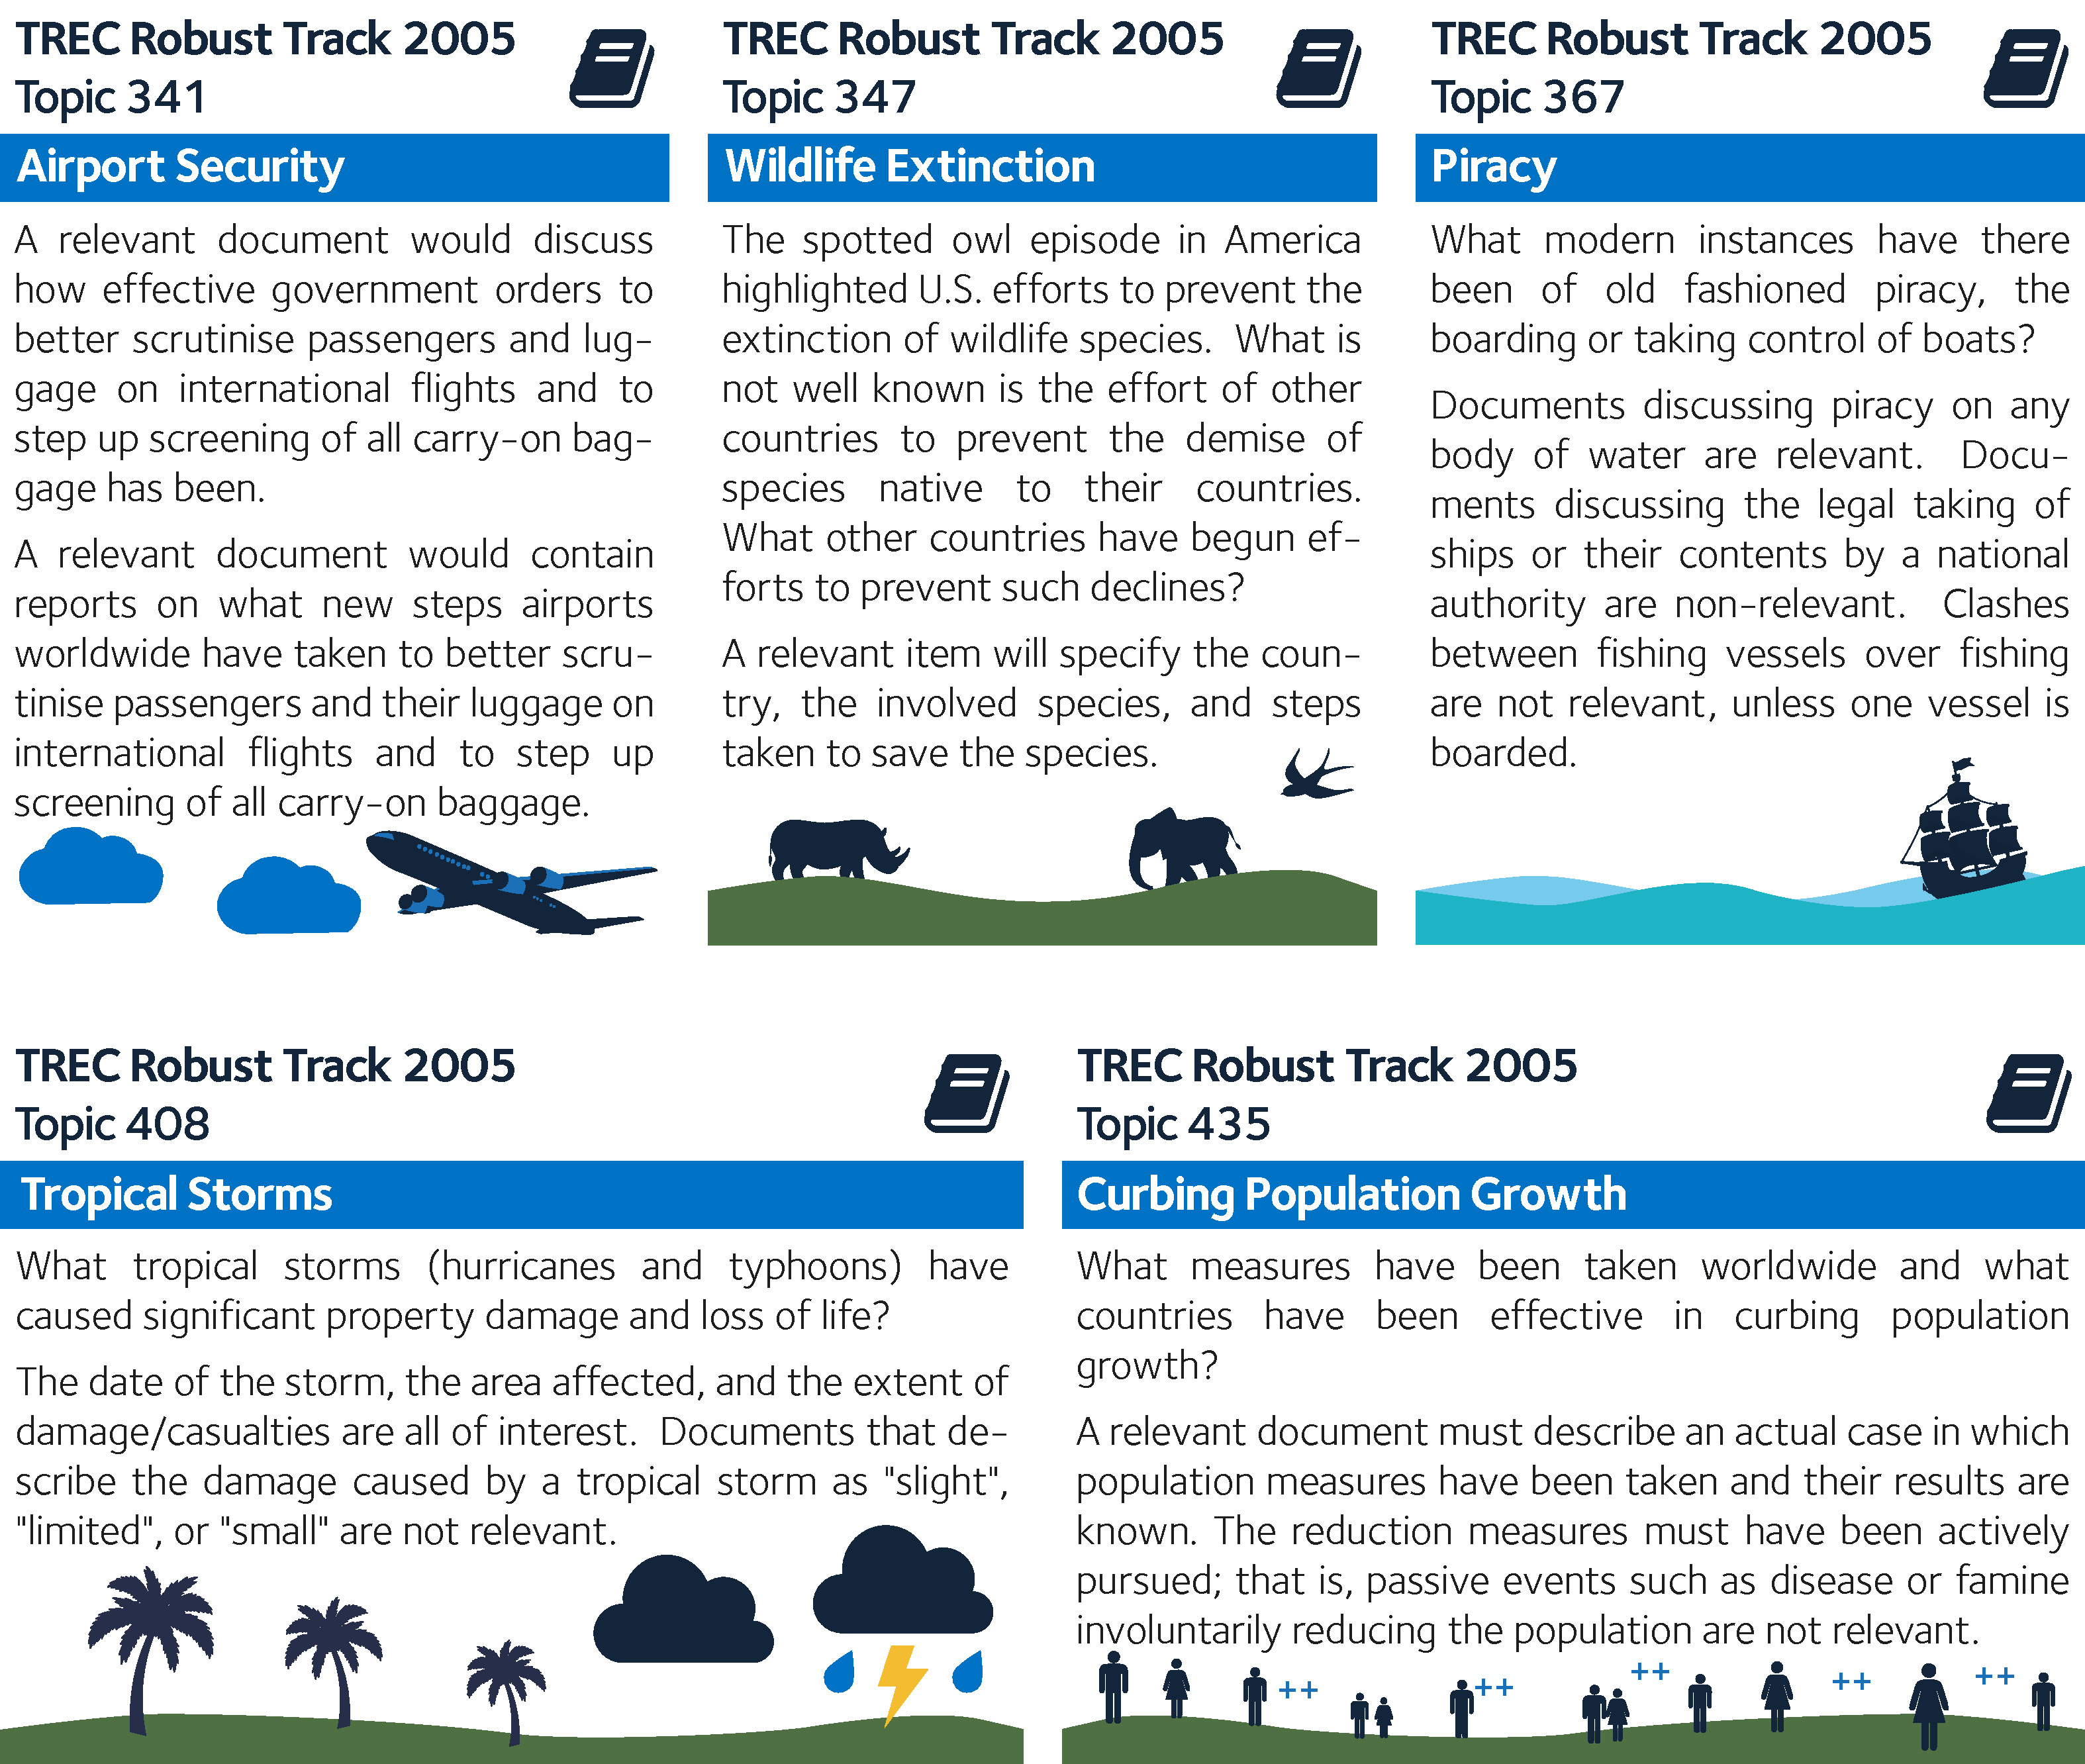
\includegraphics{figures/ch4-topics.pdf}}
    \caption[Examples of TREC Topics]{Three examples of \emph{TREC topic descriptions}, as outlined in Section~\ref{sec:csm:csm:flow}. Topics are extracted from the \emph{TREC 2005 Robust Track,} as outlined by~\cite{voorhees2006trec_robust}. Descriptions provide an explanation as to what constitutes a relevant (and often non-relevant) document.}
    \label{fig:topics}
\end{figure}

\begin{itemize}
    
    \item[]{\blueboxbold{Topic 341 – Airport Security} This topic considers relevant documents as those that discuss additional security measures that were taken by international airports around the world. Relevance is only denoted when a document discusses measures that go beyond the basic passenger and carry-on luggage screening. For example, AQUAINT document \texttt{NYT19980616.0123} discusses \emph{San Francisco International Airport's} attempts at introducing a \emph{robot sniffer,} attempting to look for nitroglycerine in luggage.}
    
    \item[]{\blueboxbold{Topic 347 – Wildlife Extinction} As the title of the topic suggests, this topic concerns wildlife extinction, and what efforts have been taken by countries other than the United States to counter the decline in endangered wildlife. Relevant documents explicitly mention the country, the species of animal, and the efforts the state or other governmental agency took to prevent decline in numbers. For example, document \texttt{XIE20000531.0205} discusses the breeding programme undertaken by China to bolster the number of Siberian Tigers in its jurisdiction.}
    
    \item[]{\blueboxbold{Topic 367 – Piracy} Instances of modern piracy are considered relevant to this topic -- not in the sense of software piracy, but the act of a water going vessel being boarded by individuals wishing to hijack it. Document \texttt{APW19980601.1065} provides an example of this -- the \emph{Petro Ranger}, a large fuel tanker, was boarded by pirates in 1998 in the South China Sea. To be relevant to the topic, the name of the vessel and the body of water it was hijacked on must be mentioned -- those discussing instances of when states intercepted vessels are not relevant.}
    
    \item[]{\blueboxbold{Topic 408 – Tropical Storms} Documents discussing major tropical storms are to be considered relevant, where the storm is reported to have caused significant damage and a large number of casualties. This is a particularly timely topic for the document corpus considered, as the 1998 hurricane season in the Caribbean has been reported to be one of the most costly -- both in terms of damage caused and lives lost -- in history.\footnote{This is reported by the US \emph{National Oceanic and Atmospheric Administration (NOAA),} as seen at \url{http://www.outlook.noaa.gov/98hurricanes/} -- last accessed May 15\textsuperscript{th}, 2018.} Document \texttt{APW19980921.1265} for example discusses the effects on Puerto Rico of Hurricane Georges in September 1998, leaving -- at the time of reporting -- three dead, many houses damaged, and thousands homeless.}
    
    \item[]{\blueboxbold{Topic 435 – Curbing Population Growth} The final topic considers efforts that have been made by countries around the world to control the ever increasing human population. Documents discussing this issue are only relevant to the topic if the results to a case have been made public, and a reduction in population has been actively pursued. The document must mention the country, the As such, events like famines are not relevant. A perhaps well known example of such a phenomenon is the one child policy that was pursued by China in the late 20\textsuperscript{th} century. Document \texttt{NYT19981031.0070} discusses the Chinese government's efforts to curb its expanding population at the time, with sexual education and heavy financial penalties for additional children. These efforts were shown to lead to a reduction in population, although whether this actually occurred is open to debate.}
    
\end{itemize}

For all user studies reported in this thesis, we selected topic \blueboxbold{367} as a \emph{practice topic,} permitting the participating subjects to familiarise themselves with the experimental system used. As such, we do not report any results from interactions that took place with this topic -- comparisons between simulated and actual searcher behaviours are also omitted. 

All queries submitted during experiments were also handled with the \emph{Whoosh~\gls{acr:ir} Toolkit}.\footnote{\emph{Whoosh} can be freely acquired using the \texttt{pip} \emph{Python} package manager -- documentation for Whoosh is available online at \url{http://whoosh.readthedocs.io/en/latest/intro.html} (last accessed May 15\textsuperscript{th}, 2018). The corpus was indexed with Whoosh \texttt{2.7.4}.} Using the toolkit, we indexed the AQUAINT document collection, applying Porter stemming. Stopwords -- from Fox's classical stopword list -- were also removed (refer to Section~\ref{sec:ir_background:basics:indexing} for more information on the indexing process). For this index, we also removed documents with \todo{duplicate titles}. This is an issue, especially with documents originating from a newswire. A document discussing an ongoing event may be continually revised as new information arises, leading to multiple revisions. \todo{For documents with duplicate titles, we retained the document with the latest timestamp.}

With an index weighing in at 800MB, consisting of $128,894$ documents. \todo{What else did we do to reduce this number?} We could then issue queries against the index. All ranked results from queries were computed with the BM25 algorithm, where $\beta=0.75$. Terms in the queries issues were implicitly \texttt{AND}ed together to restrict the set of retrieved documents to those that only contained all of the query terms. This was chosen to reduce the size of the returned set -- most search systems employ such an implicit approach.

\subsection{Conducting a User Study}
Using the document collection, topics and search engine defined above, our methodology then moved to conducing a user study. These studies are discussed in depth in Chapters~\ref{chap:snippets} and~\ref{chap:diversity}. While the intricate details of each study's methodology (and therefore overall goal) do differ extensively, there are nevertheless some common components that we can discuss here. The two studies consider how the behaviour, performance and perceived experiences of searchers varies when:

\begin{itemize}
    \item{the length of snippets are varied; and}
    \item{the diversity of results and task goal are varied.}
\end{itemize}

Specifically, the two studies consider stopping behaviour at both the snippet (via stopping strategies) and session (via goal) level. We discuss the specific interfaces and conditions that we trial in more detail in the relevant chapters.

Studies were undertaken using a custom built experimental framework called \emph{TREConomics.}\footnote{TREConomics can be found online at \url{https://github.com/leifos/treconomics} -- last accessed May 15\textsuperscript{th}, 2018.} The framework has been developed over a number of years, and has been successfully deployed over a number of studies, including those by~\cite{azzopardi2013query_cost},~\cite{maxwell2014temporal_delays} and~\cite{kelly2015serp_size}.

Within-subjects design...

\subsubsection{Experimental Flow}\label{sec:csm:methodology:user:flow}
demo
practice
task
surveys

\subsubsection{Experimental Interface}
Screenshot of the experimental interface

\subsubsection{Capturing Interactions}
Produces a log file, that captures a number of different interactions with the search engine.

\subsubsection{Crowdsourcing}
For both studies highlighted above, we employed a \emph{crowdsourced} approach to our experimentation. As highlighted by Zuccon et al.~\cite{zuccon2013crowdsourcing}, crowdsourcing provides an alternative means for capturing user interactions and search behaviours from traditional lab-based user studies. Greater volumes of data can be obtained from more heterogeneous workers at a lower cost -- all within a shorter timeframe. Of course, pitfalls of a crowdsourced approach include the possibility of workers completing tasks as efficiently as possible, or submitting their tasks without performing the requested operations~\cite{feild2010turkers}. Despite these issues, it has been shown that there is little difference in the quality between crowdsourced and lab-based studies~\cite{zuccon2013crowdsourcing}. Nevertheless, quality control is a major component of a well-executed crowdsourced experiment~\cite{bota2016playing_your_cards}. Here, we detail our subjects and precautions taken.

The study was run over the \emph{Amazon Mechanical Turk (MTurk)} platform. Workers from the platform performed a single \emph{Human Intelligence Task (HIT)}, which corresponded to the entire experiment. Due to the expected length of completion for the study (45-50 minutes), subjects who completed the study in full were reimbursed for their time with US\$9; a typically larger sum (and HIT duration) than most crowdsourced experiments. We examined extra precautionary measures to ensure the integrity of the log data that was recorded. Precautions were taken from several angles. First, workers were only permitted to begin the experiment on the MTurk platform that: \emph{(i)} were from the United States, and were native English speakers; \emph{(ii)} had a HIT acceptance rate of at least 95\%; and \emph{(iii)} had at least 1000 HITs approved. Requiring \emph{(ii)} and \emph{(iii)} reduced the likelihood of recruiting individuals who would not complete the study in a satisfactory manner. Recruits were forewarned about the length of the HIT, which was considerably longer than other crowdsourced experiments.

We also ensured that the computer the subject was attempting the experiment on had a sufficiently large screen resolution (1024x768 or greater) so as to display all of the experimental interface on screen. With the experiment being conducted in a Web browser popup window of a fixed size, we wanted to ensure that all subjects would be able to see the same number of results on a SERP within the popup window's viewport. As the experiment was conducted via a Web browser, we wanted to ensure that only the controls provided by the experimental apparatus were used, meaning that the popup window had all other browser controls disabled to the best of our ability (i.e. history navigation, etc.). The experimental system was tested on several major web browsers, across different operating systems. This gave us confidence that a similar experience would be had across different system configurations.

For each of the different interfaces and conditions that we trialled, a number of post-processing scripts were implemented to record a variety of different information that we discuss below.

\todo{Need to mention interaction log}

\subsection{Extracting User Study Interaction Data}\label{sec:csm:methodology:extracting}
With the TREConomics framework providing the necessary infrastructure allowing us to capture a variety of different behavioural and experience characteristics, we now detail what aspects we consider. Figure~\ref{fig:evaluation_methodology} provides examples of the different aspects we consider, being split into four different categories.

The first three categories can be extracted directly from the interaction log that recorded different interactions by each subject as they progressed through the experiment. The categories we considered are listed below.

\begin{itemize}
    
    \item[]{\blueboxbold{Interactions} capture the broad interactions that take place, such as clicks.}
    \item[]{\blueboxbold{Performance} measures could be extrapolated, with aid of TREC QREL relevance judgements, to ascertain the performance of subjects.}
    \item[]{\blueboxbold{Time-Based} measures can also be derived from directly examining the interaction log, measuring the time spent between different logged interactions.}
    
\end{itemize}

In addition to these categories, we also observed a number of \blueboxbold{user experience} measures that are derived from a series of surveys that subjects were presented with as they were walked through the experimental process. In particular, as highlighted in Section~\ref{sec:csm:methodology:user:flow}, surveys were presented to subjects at a number of different stages throughout the experiment. In conjunction with the three log-based categories defined above, the user experience measures could be used to complement the empirical evidence to see whether the interactions of subjects actually correlated with their perceived experiences.

In all, the interactions -- including aspects such as clicks, and time-based measures, were used as a \emph{grounding} for our subsequent user simulations. These are discussed in Section~\ref{chap:csm:method:simulation} and derived for each experimental condition and interface trialled.

\begin{figure}[t!]
    \centering
    \resizebox{1\hsize}{!}{
    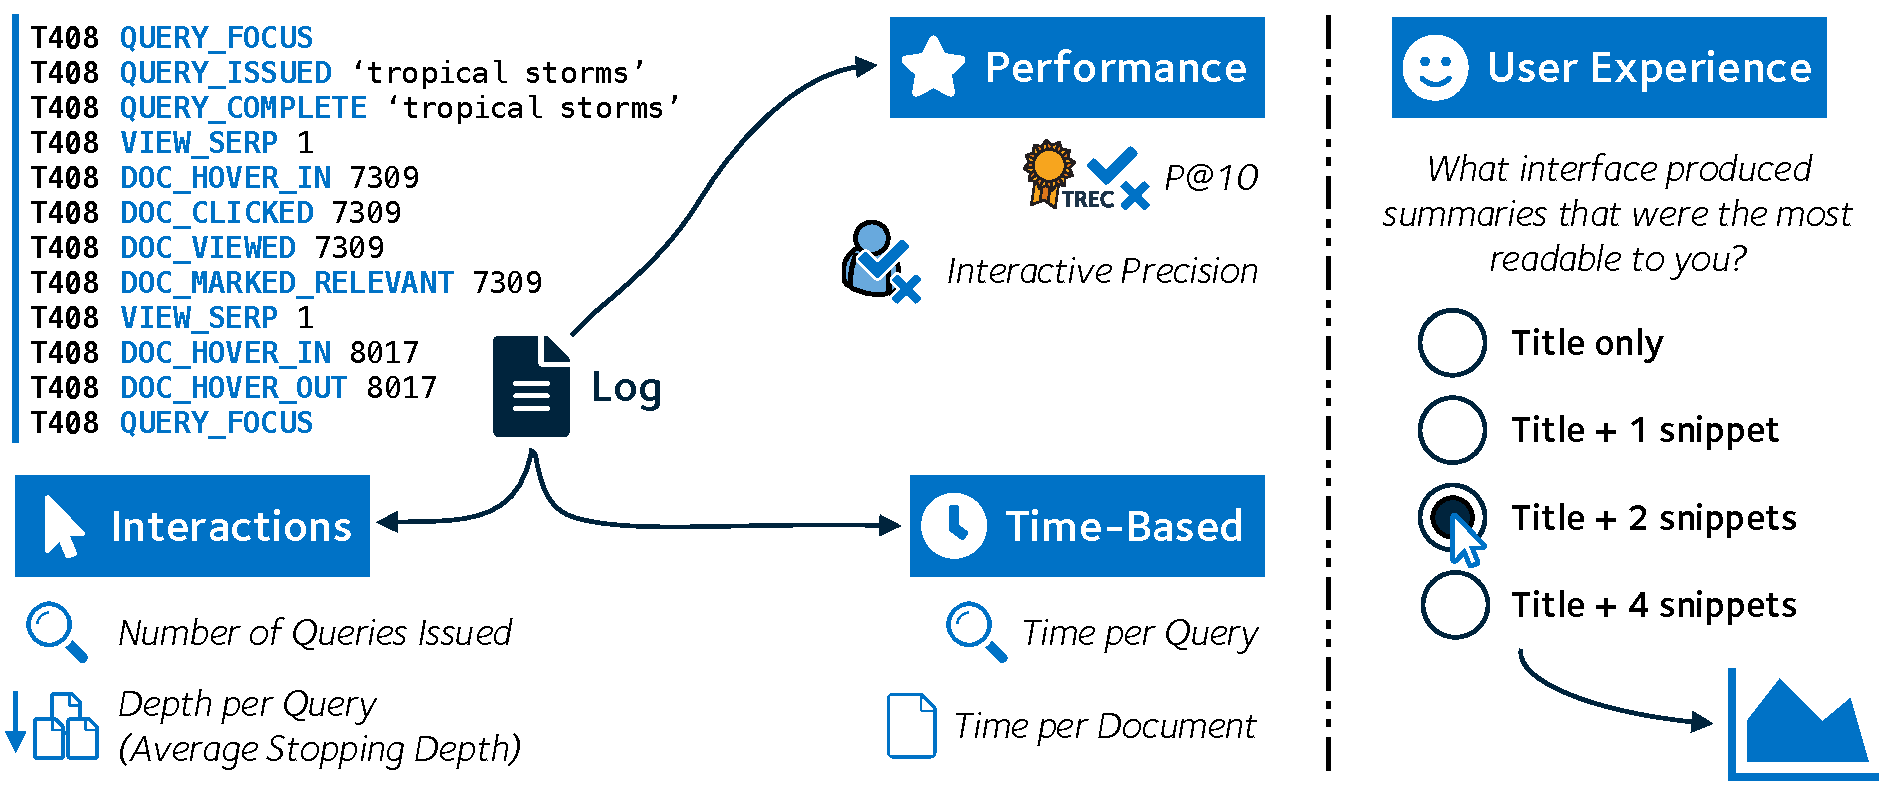
\includegraphics{figures/ch4-evaluation.pdf}}
    \caption[Examples of Evaluation Measures]{An illustration of the different types of measures that are captured, and from what sources. Interaction, time-based and performance measures are derived from the user study experiment log (with TREC QRELs used in conjunction with the interaction log to compute a subject's performance). User experience metrics are collated from a number of different surveys. Refer to Section~\ref{sec:csm:methodology:extracting} for more information.}
    \label{fig:evaluation_methodology}
\end{figure}

\subsubsection{Basic Interactions}
- recorded from log data.
- a number of different behavioural measures were recorded!

- clicks
- hovers
- and from that, the click depths. only click depths -- see time-based measures for an explanation as to why this is the case.
- number of queries
- number of documents marked

- list from the papers.

\subsubsection{Time-Based Measures}
- from the log data, as mentioned above, we also derived a number of time based measures.

- calculated from the point at which a searcher clicks or whatever, to the point they begin to do something else.

- query time -- from focus, to issuance.

- document time -- from clicking on a document, to returning to the~\gls{acr:serp}.

- per snippet time -- originally calculated from hover events. however, this in both studies proved to be unreliable.
- events triggered an AJAX callback...these came back to the server in a different order from which they were sent from the client, in a random order. as such, logging was inconsistent. and difficult to parse, unreliable.

- so made assumptions instead. we instead looked purely at the click depths for stopping -- and ignored hovers. use these for stopping depths.

\subsubsection{Performance Measures}
- as shown from figure~\ref{}, we were also able to extract a number of performance measures, too.
- using the raw data extracted from the interaction log file, we could, in conjunction with an additional evaluation tool (i.e. trec\_eval), use these two resources to calculate measures.

- measures that we considered across both studies included:

- P@10 -- query-based measures
- interactive precision and recall
- considering things too like number of documents marked, yet are not relevant.

- used in conjunction with behavioural measures, formed the basis of the seeded experiments.

\subsubsection{User Experience}
- not strictly necessary to forming a grounded simulation.
- but included to ascertain whether subjects perceived a difference between the interfaces and conditions trialled across the two experiments.

- split into five main parts:
    - demographics
    - pre-experiment
    - pre-task
    - post-task
    - post-experiment

- as previously mentioned, many of these components differed across the two studies that were undertaken. as such, we leave explanation of these surveys to each of the chapters.

\subsection{Simulating Searcher Behaviours}\label{chap:csm:method:simulation}
Simulation as defined earlier is a good means for experimentation.
Low cost, always use the same users, no issue of learning bias, etc.

EXPLORE how people's behaviours change

- set up the probabilities
- instantiate the components

- pick a topic set
- pick a corpus
- basic structure of the methodology from previous papers

\subsubsection{Instantiating the Simulations}

\subsubsection{Performance Runs}

\subsubsection{Comparison Runs}

\subsection{Evaluation of Simulations}\label{chap:csm:method:evaluation}
- how do we evaluate how good the system performs?
- how do we work out which one approximates best? on average.

\subsubsection{Determining Simulated User Performance}

\subsubsection{Comparing Simulated and Real-World Subjects}

\section{Chapter Summary}